\documentclass[aspectratio=169]{beamer}
\usepackage[utf8]{inputenc}
\usepackage{tikz}
\usepackage{tikz-cd}
\usepackage{tikz-layers}
\usepackage{pifont}
\usepackage{pgfpages}
\usepackage{pgfplots}
\usepackage{graphicx}
\usepackage[export]{adjustbox}
\usepackage{qrcode}
\usepackage{caption}
\usepackage{minted}
\usepackage[svgnames]{xcolor}
\usetikzlibrary{backgrounds}
\usetikzlibrary{decorations.pathreplacing}

% the drgtheme files live once at the repo root, in ../../../theme/
\makeatletter
\def\input@path{{../../../theme/}}
\makeatother
\graphicspath{{../images/}{../../../theme/}}

\usetheme{drgtheme}

%setup cover page variables
\title{MAC 233: Hall Effect Sensor Lab}
\author{
    Dr Max Champneys
}
\institute[UoS]{
    School of Mechanical, Aerospace, and Civil Engineering,\\
    University of Sheffield, UK
}
\date{MAC 233: \hspace{0.1em}\textbf{04/11/2026}}
%setup footer variables
\runninginstitute{MAC 233, School of MAC, University of Sheffield}
\email{max.champneys@sheffield.ac.uk}

%Begin Document
\begin{document}

%Create Title Page
\maketitle

\begin{frame}{MAC 233: Labs Overview}
    \begin{center}
        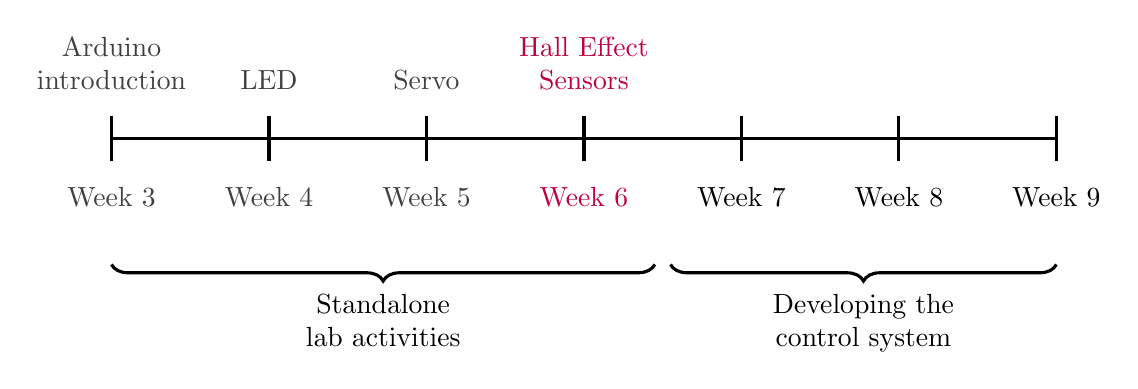
\begin{tikzpicture}[
            timeline/.style={color=black, line width=0.4mm},
            pastnode/.style={align=center, color=darkgray},
            currentnode/.style={align=center, color=purple},
            futurenode/.style={align=center, color=black}
        ]
            %line
            \draw[timeline] (-6, 0) -- (6, 0);

            % week ticks
            \foreach \x in {-6, -4, -2, 0, 2, 4, 6}{
                \draw[timeline] (\x, -0.28) -- (\x, 0.28);
            }

            % weeks (below the line)
            \node[pastnode, below] at (-6, -0.5) {Week 3};
            \node[pastnode, below] at (-4, -0.5) {Week 4};
            \node[pastnode, below] at (-2, -0.5) {Week 5};
            \node[currentnode, below] at (0, -0.5) {Week 6};
            \node[futurenode, below] at (2, -0.5) {Week 7};
            \node[futurenode, below] at (4, -0.5) {Week 8};
            \node[futurenode, below] at (6, -0.5) {Week 9};

            % activities (above the line)
            \node[pastnode, above] at (-6, 0.5) {Arduino\\introduction};
            \node[pastnode, above] at (-4, 0.5) {LED};
            \node[pastnode, above] at (-2, 0.5) {Servo};
            \node[currentnode, above] at (0, 0.5) {Hall Effect\\Sensors};

            % phases
            \draw[timeline, decorate, decoration={brace, amplitude=6pt, mirror}] (-6, -1.6) -- (0.9, -1.6);
            \node[futurenode, below] at (-2.55, -1.85) {Standalone\\lab activities};
            \draw[timeline, decorate, decoration={brace, amplitude=6pt, mirror}] (1.1, -1.6) -- (6, -1.6);
            \node[futurenode, below] at (3.55, -1.85) {Developing the \\ control system};

        \end{tikzpicture}
    \end{center}
\end{frame}

\begin{frame}{Today's Lab: Prerequisites}
    \Large
    This lab doesn't require any code from previous labs; however, it does expect you to have completed these, as common code repeated from previous labs will not be explained in detail again here.\\
    
    Out of your Arduino pack, you will need: 1 Arduino, 1 breadboard, 1 A3144 hall effect sensor, 1 magnet, 1 LED, 1 $10K\Omega$ resistor, 1 $220\Omega$ resistor, and 5 jumper cables.
\end{frame}

\begin{frame}{Today's Lab: Objectives}
    \Large
    The objective of today's lab is to learn how to use an interrupt to record a value of a Hall effect sensor when a magnet passes it.
    \vspace{.5em}
    
    \url{https://docs.arduino.cc/language-reference/en/functions/external-interrupts/attachInterrupt/}.
\end{frame}

\begin{frame}{Reading an input: why we need an interrupt}
    \begin{center}
        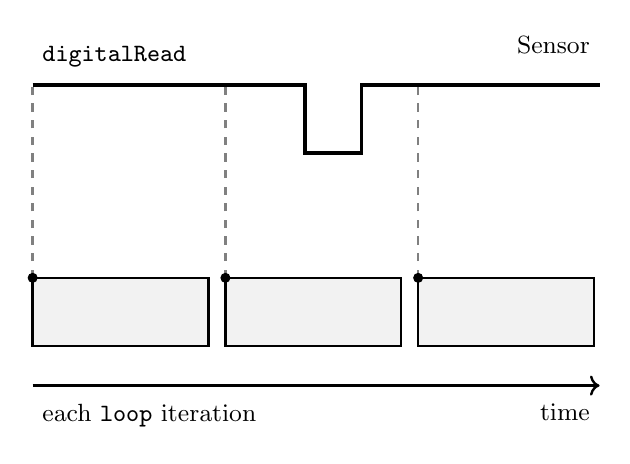
\begin{tikzpicture}[
            x=.72cm, y=.72cm,
            signal/.style={line width=.5mm},
            iter/.style={line width=.3mm, fill=black!5},
            readline/.style={dashed, draw=gray, line width=.3mm},
            lbl/.style={font=\small},
        ]
            %% polling: the pin is only read at the start of each iteration
            \node[lbl, anchor=east] at (10, 5.3) {Sensor};
            \draw[signal] (0, 4.6) -- (4.8, 4.6) -- (4.8, 3.4)
                -- (5.8, 3.4) -- (5.8, 4.6) -- (10, 4.6);

            \node[lbl, anchor=south west] at (0, 4.75) {\texttt{digitalRead}};
            \foreach \s in {0, 3.4, 6.8}{
                \draw[iter] (\s, 0) rectangle ++(3.1, 1.2);
                \draw[readline] (\s, 1.2) -- (\s, 4.6);
                \filldraw (\s, 1.2) circle (1.6pt);
            }

            \draw[->, line width=.3mm] (0, -0.7) -- (10, -0.7);
            \node[lbl, anchor=north east] at (10, -0.85) {time};
            \node[lbl, anchor=north west] at (0, -0.85) {each \texttt{loop} iteration};
        \end{tikzpicture}
    \end{center}

    \vspace{.5em}
    An input can change at any moment, but the `loop' function only looks at it once per iteration. A magnet that comes and goes in between is never seen.
\end{frame}

\begin{frame}{Reading an input: the interrupt}
    \begin{center}
        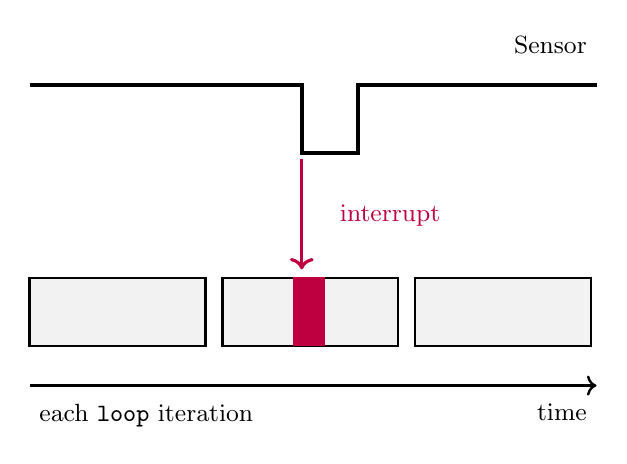
\begin{tikzpicture}[
            x=.72cm, y=.72cm,
            signal/.style={line width=.5mm},
            iter/.style={line width=.3mm, fill=black!5},
            lbl/.style={font=\small},
        ]
            %% the falling edge interrupts the loop the moment it happens
            \node[lbl, anchor=east] at (10, 5.3) {Sensor};
            \draw[signal] (0, 4.6) -- (4.8, 4.6) -- (4.8, 3.4)
                -- (5.8, 3.4) -- (5.8, 4.6) -- (10, 4.6);

            \foreach \s in {0, 3.4, 6.8}{
                \draw[iter] (\s, 0) rectangle ++(3.1, 1.2);
            }

            \filldraw[fill=purple, draw=purple] (4.65, 0) rectangle ++(0.55, 1.2);
            \draw[->, line width=.4mm, draw=purple] (4.8, 3.3) -- (4.8, 1.35);
            \node[lbl, anchor=west, text=purple] at (5.3, 2.3) {interrupt};

            \draw[->, line width=.3mm] (0, -0.7) -- (10, -0.7);
            \node[lbl, anchor=north east] at (10, -0.85) {time};
            \node[lbl, anchor=north west] at (0, -0.85) {each \texttt{loop} iteration};
        \end{tikzpicture}
    \end{center}

    \vspace{.5em}
    An interrupt pauses the `loop' function the moment the pin changes, runs a function of your choosing, and then carries on where it left off.
\end{frame}

% [fragile] is required for the inline minted listing
\begin{frame}[fragile]{New: `attachInterrupt'}
    \normalsize
    One line in \verb|setup| says which pin to watch, which function to call, and when:
    \vspace{.5em}
\begin{minted}[fontsize=\footnotesize]{arduino}
attachInterrupt(digitalPinToInterrupt(CRANK_PIN), crankInterrupt, FALLING);
\end{minted}
    \vspace{.5em}
    \begin{itemize}
        \setlength{\itemsep}{.6em}
        \item \mintinline{arduino}{digitalPinToInterrupt(CRANK_PIN)} --- the pin to watch
        \item \mintinline{arduino}{crankInterrupt} --- the function to call, with no brackets
        \item \mintinline{arduino}{FALLING} --- when: as the pin drops from 5\,V to 0\,V
    \end{itemize}
\end{frame}

% [fragile] is required for the inline minted listing
\begin{frame}[fragile]{New: the interrupt function}
    \normalsize
    The function you named is an ordinary function, written beside \verb|setup| and \verb|loop| --- never inside them:
    \vspace{.5em}
\begin{minted}[fontsize=\small]{arduino}
void crankInterrupt() {
  crank_interrupt_current_time = millis();
}
\end{minted}
    \vspace{.5em}
    It runs the moment the magnet arrives, whatever the `loop' function was part-way through. Keep it as short as you can: record what you need, and get out.
\end{frame}

% [fragile] is required for the inline minted listing
\begin{frame}[fragile]{Variables: `volatile'}
    \Large
    An interrupt can change a variable at any moment. Marking it `volatile' tells the compiler not to cache the value, so the main `loop' always sees what the interrupt wrote.
    \vspace{.75em}
\begin{minted}[fontsize=\small]{arduino}
// written by the interrupt, read by the loop
volatile unsigned long crank_interrupt_current_time;

// only ever touched by the loop, so no volatile
unsigned long current_loop_time;
\end{minted}
\end{frame}

\begin{frame}{Wiring Diagram}
    \vspace{-.5em}
    \begin{center}
        \begin{tikzpicture}[
            scale=1.65, transform shape, rotate=90,
            wire/.style={line width=.8mm},
            leg/.style={draw=DimGray},
            jumper/.style={draw=LimeGreen},
        ]


            %% mask out breadboard
            \filldraw[fill=white, draw=white] (-.62, -1.49) rectangle (-.44, -0.98);

            %% legs 5 per span y = 0.188, per span x = 0.183
            \draw[wire, leg] (.975,-0.515) -- (.975, 1.16); %220 resistor
            \draw[wire, leg] (.792,-1.61) -- (.792, -0.49);%led
            \draw[wire, leg] (-.495,-1.61) -- (-.495, -0.86);%hall effect
            \draw[wire, leg] (-.69,-1.23) -- (-.59, -1.23);%hall effect
            \draw[wire, leg] (-.865,-1.61) -- (-.865, -0.86);%10k resistor

            %% cables
            \draw[wire, jumper] (.607,-1.61) -- (.607, 0.604);
            \draw[wire, jumper] (-1.05,-1.244) -- (-1.05, 0.238);
            \draw[wire, jumper] (-.31,-0.88) -- (-.31,-0.32) -- (-.865,-0.32) -- (-.865, 0.604);
            \draw[wire, jumper] (-.31,-1.61) -- (.422,-1.61) -- (.422,-0.307) to[out=50, in=130] (.792,-0.307) -- (.792, 0.792);

            %% components
            \node[] at (-.865, -1.23) {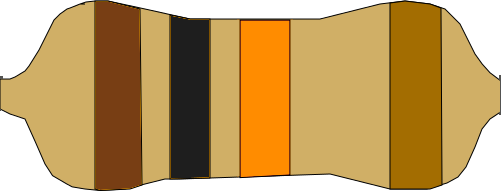
\includegraphics[angle=90, origin=c,width=1.75mm]{../images/resistor-10k.png}}; %10k resistor
            \fill[fill=red] (-.44,-1.44) -- (-.44, -1.04) -- (-.54, -1.04) -- (-.59, -1.14) -- (-.59, -1.34) -- (-.54, -1.44) -- cycle; %hall effect
            \filldraw[fill=red, draw=black] (.79,-1.05) circle (1.25mm); %led
            \node[] at (.975, 0.323) {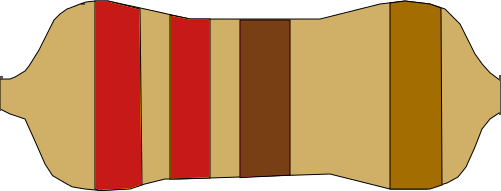
\includegraphics[angle=90, origin=c,width=1.75mm]{../images/resistor-220.png}}; %220 resistor
            \node[] at (-.13, 1.43) {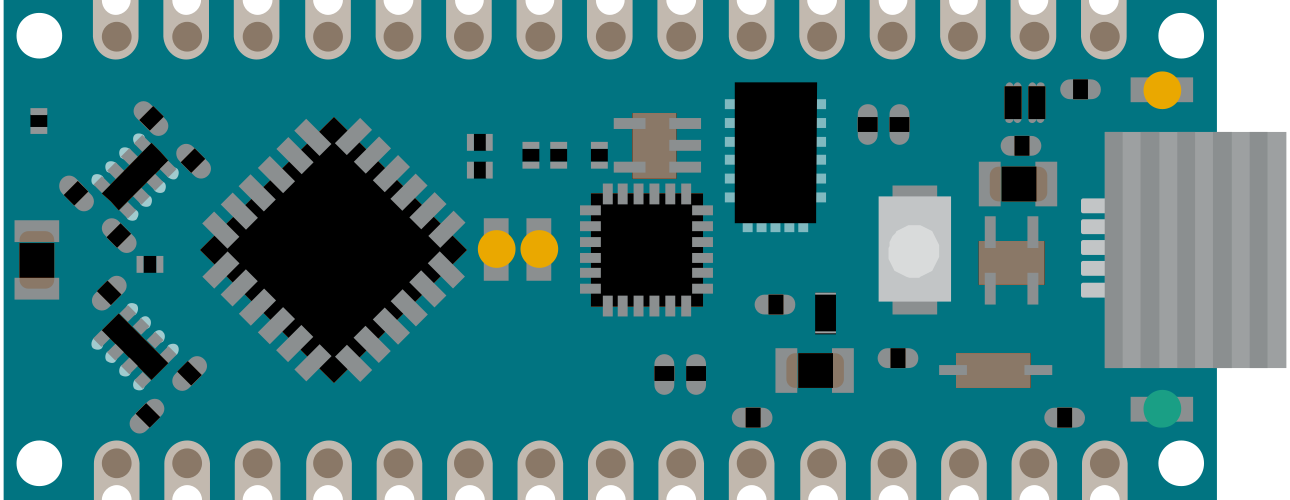
\includegraphics[angle=90, origin=c, width=3.38em]{../images/nano.png}}; %nano

            %% breadboard background
            \begin{scope}[on background layer]
                \node[] at (0, 0) {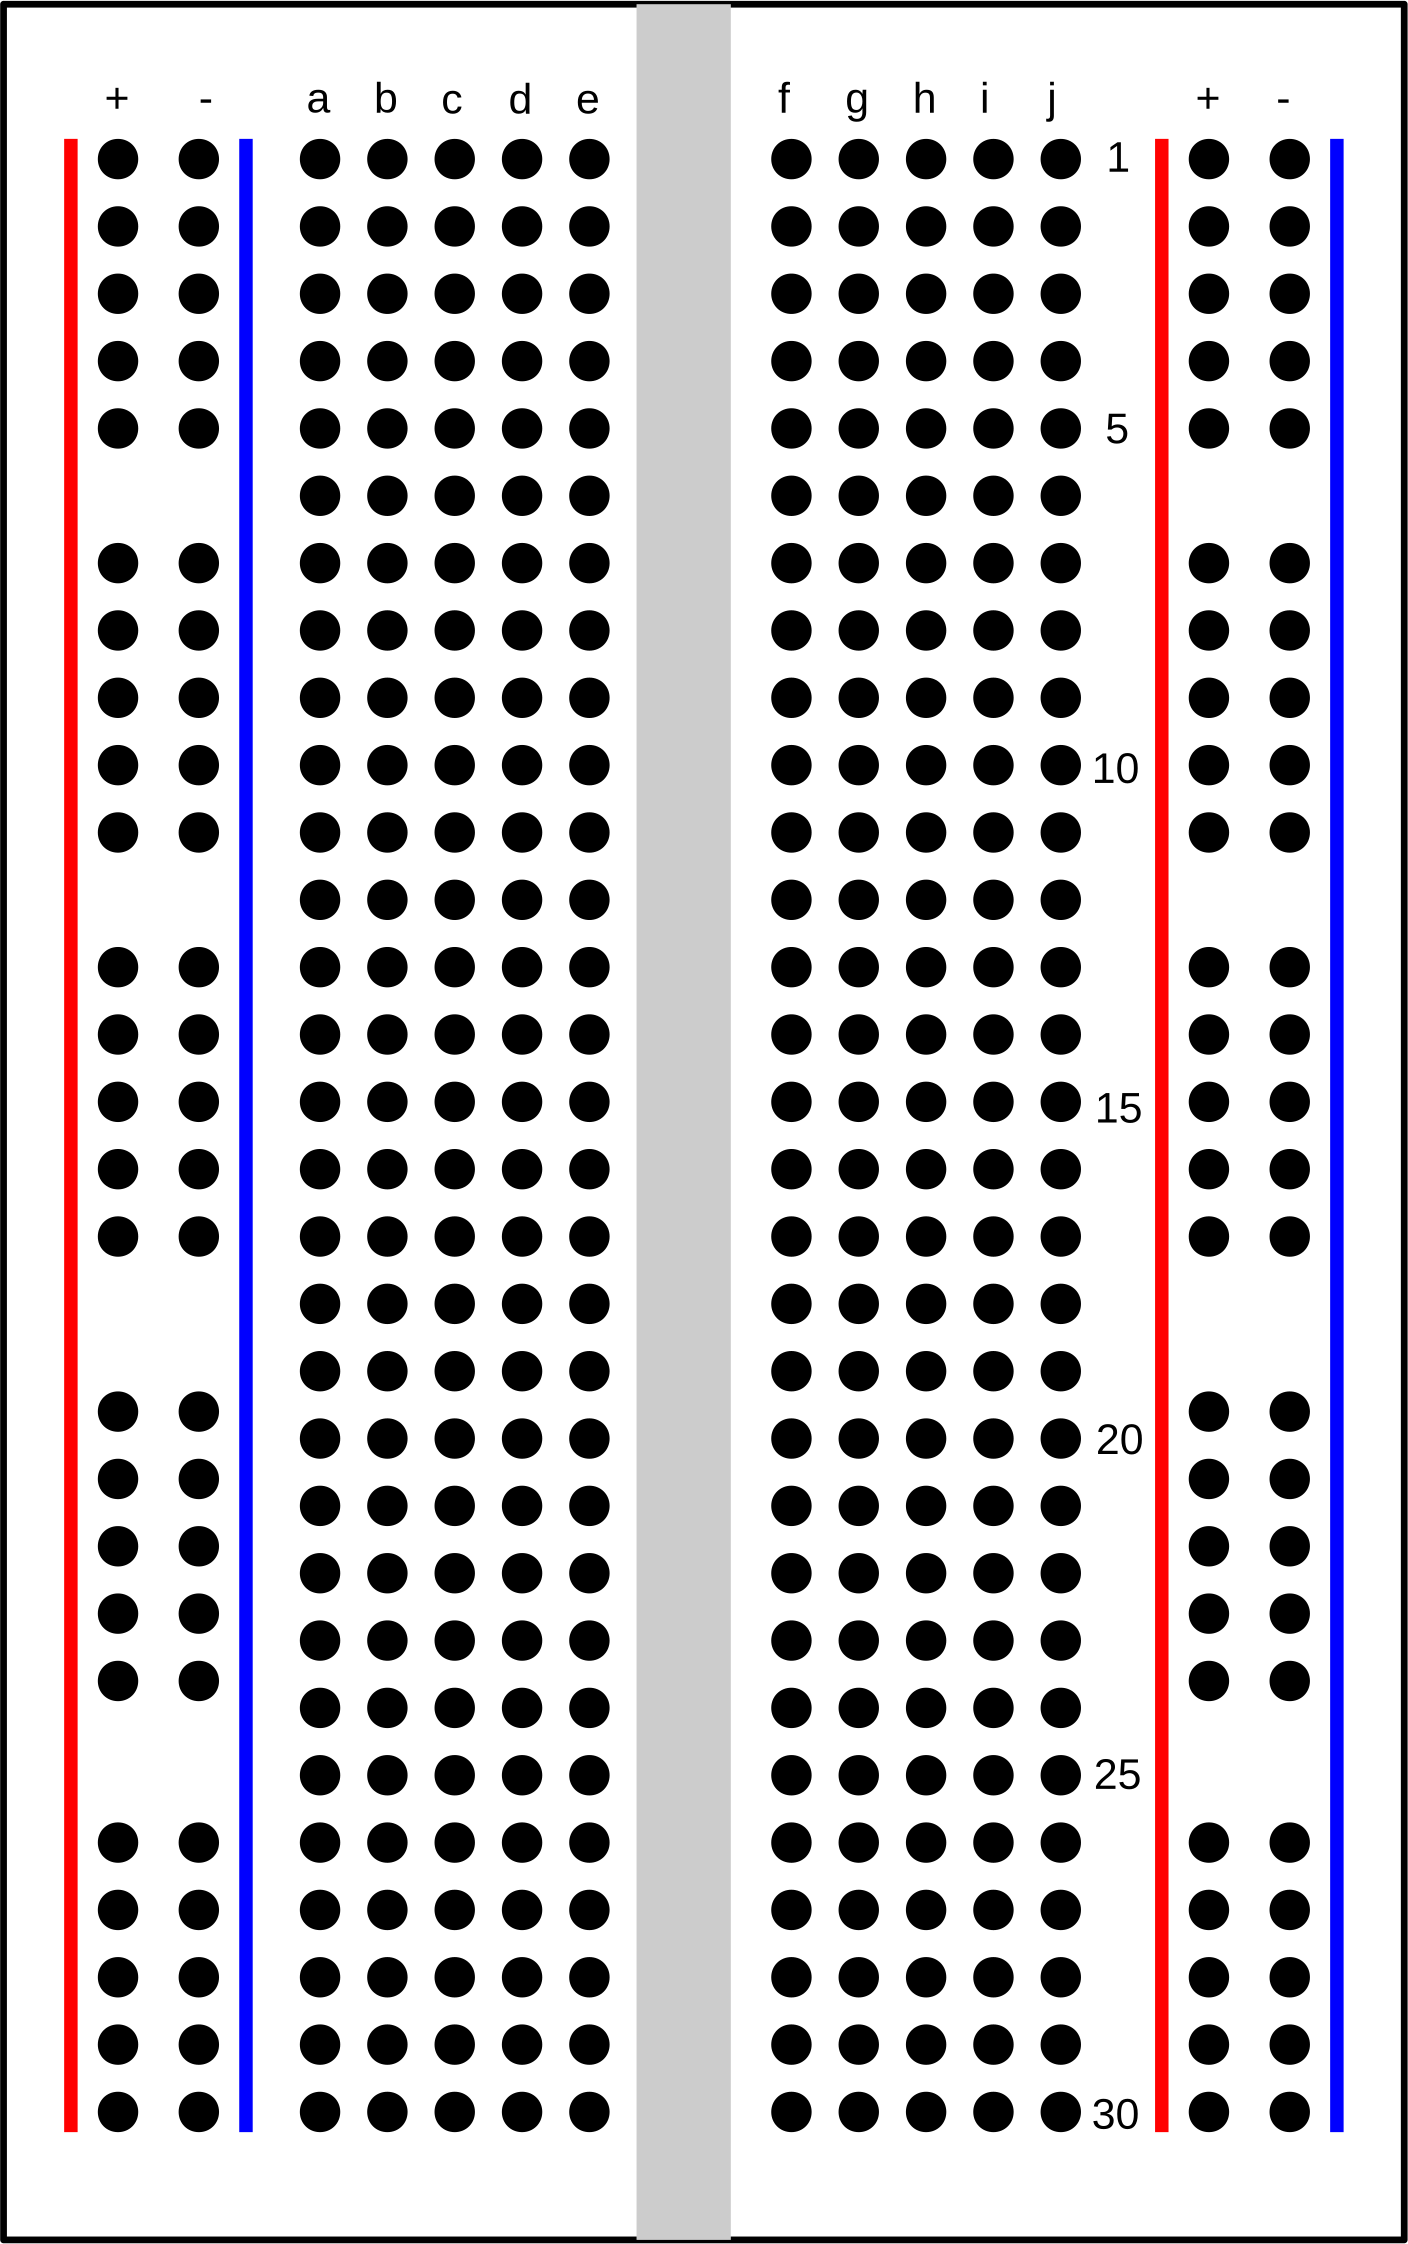
\includegraphics[width=10em]{../images/breadboard.png}};
            \end{scope}

        \end{tikzpicture}
    \end{center}
    \tiny
    Breadboard source: \url{https://freesvg.org/breadboard}, Resistor source \url{https://freesvg.org/resistor-330-ohm}.
\end{frame}

\begin{frame}{Help}
    \Large

    \normalsize
    \begin{columns}
        \begin{column}{.5\textwidth}
            \begin{center}
                \textbf{Lab 4 worksheet}\\
                \vspace{.5em}
                \qrcode[hyperlink, height=3cm]{https://github.com/MDCHAMP/MAC233/blob/main/labs/lab-4-hall-effect-sensor/docs/lab-4-hall-effect-sensor.pdf}
            \end{center}
        \end{column}
        \begin{column}{.5\textwidth}
            \begin{center}
                \textbf{Nano Every pinout}\\
                \vspace{.5em}
                \qrcode[hyperlink, height=3cm]{https://docs.arduino.cc/resources/pinouts/ABX00028-full-pinout.pdf}
            \end{center}
        \end{column}
    \end{columns}


    \vspace{3.5em}
    Problems? Raise your hand and someone will come and help you.

\end{frame}

\end{document}
